\documentclass{article}
\usepackage{graphicx} % Required for inserting images

\title{Mental Health Capstone Project}
\author{McKenna Roessler}
\date{February 2026}

\begin{document}

\maketitle

\section{Introduction}
We've all been impacted by mental health at some point before. Whether through personal experience, 
the experiences of friends or loved ones, or even coworkers and peers, everyone has seen what the human mind is capable of. We all experience the world, after all; just in different ways. As a student of computer science and a psychology degree holder, my goal has long been to find a way to combine my admittedly vastly different areas of interest in a way that helps people. Mental health was and is my passion within the psychology field, and although I decided graduate school for counseling or clinical psychology wasn't the right path for me, I have never lost my desire to help those in need. Luckily, psychology and computer science aren't mutually exclusive after all. Technology and computers were designed to help people. They make the things that humans do easier, and help them with daily tasks. Who's to say they can't take some of the emotional burden off our shoulders too? That's where my interest in mental health software comes into play. As we venture into the world of telehealth, chatbots, and mood trackers, the demand for convenient and accessible mental health technology is growing. While it can't replace traditional therapy, I believe software built on familiar devices we use every day can play a critical role in complementing mental health treatment. It can allow users to feel safe and comfortable, as well as feel in control of their treatment and progress. It can provide easy access to resources at the push of a button. It may even be able to predict harmful behaviors and patterns before a user or therapist can. I would like to play a role in developing these helpful tools so more people can have access to the help and resources they need. This capstone project is my first step into this field. The project takes the form of an Android phone app and allows users to track their mood every day, allowing them to compare their data over longer periods of time and pick up on patterns of symptoms. It also allows them to write out their thoughts more specifically and recommends resources and articles that may be of interest to them based on their symptoms and concerns. This application allows for a daily opportunity for users to check in with themselves, which could help them discover what further aid and resources they need.

\section{App Layout}
Homescreen

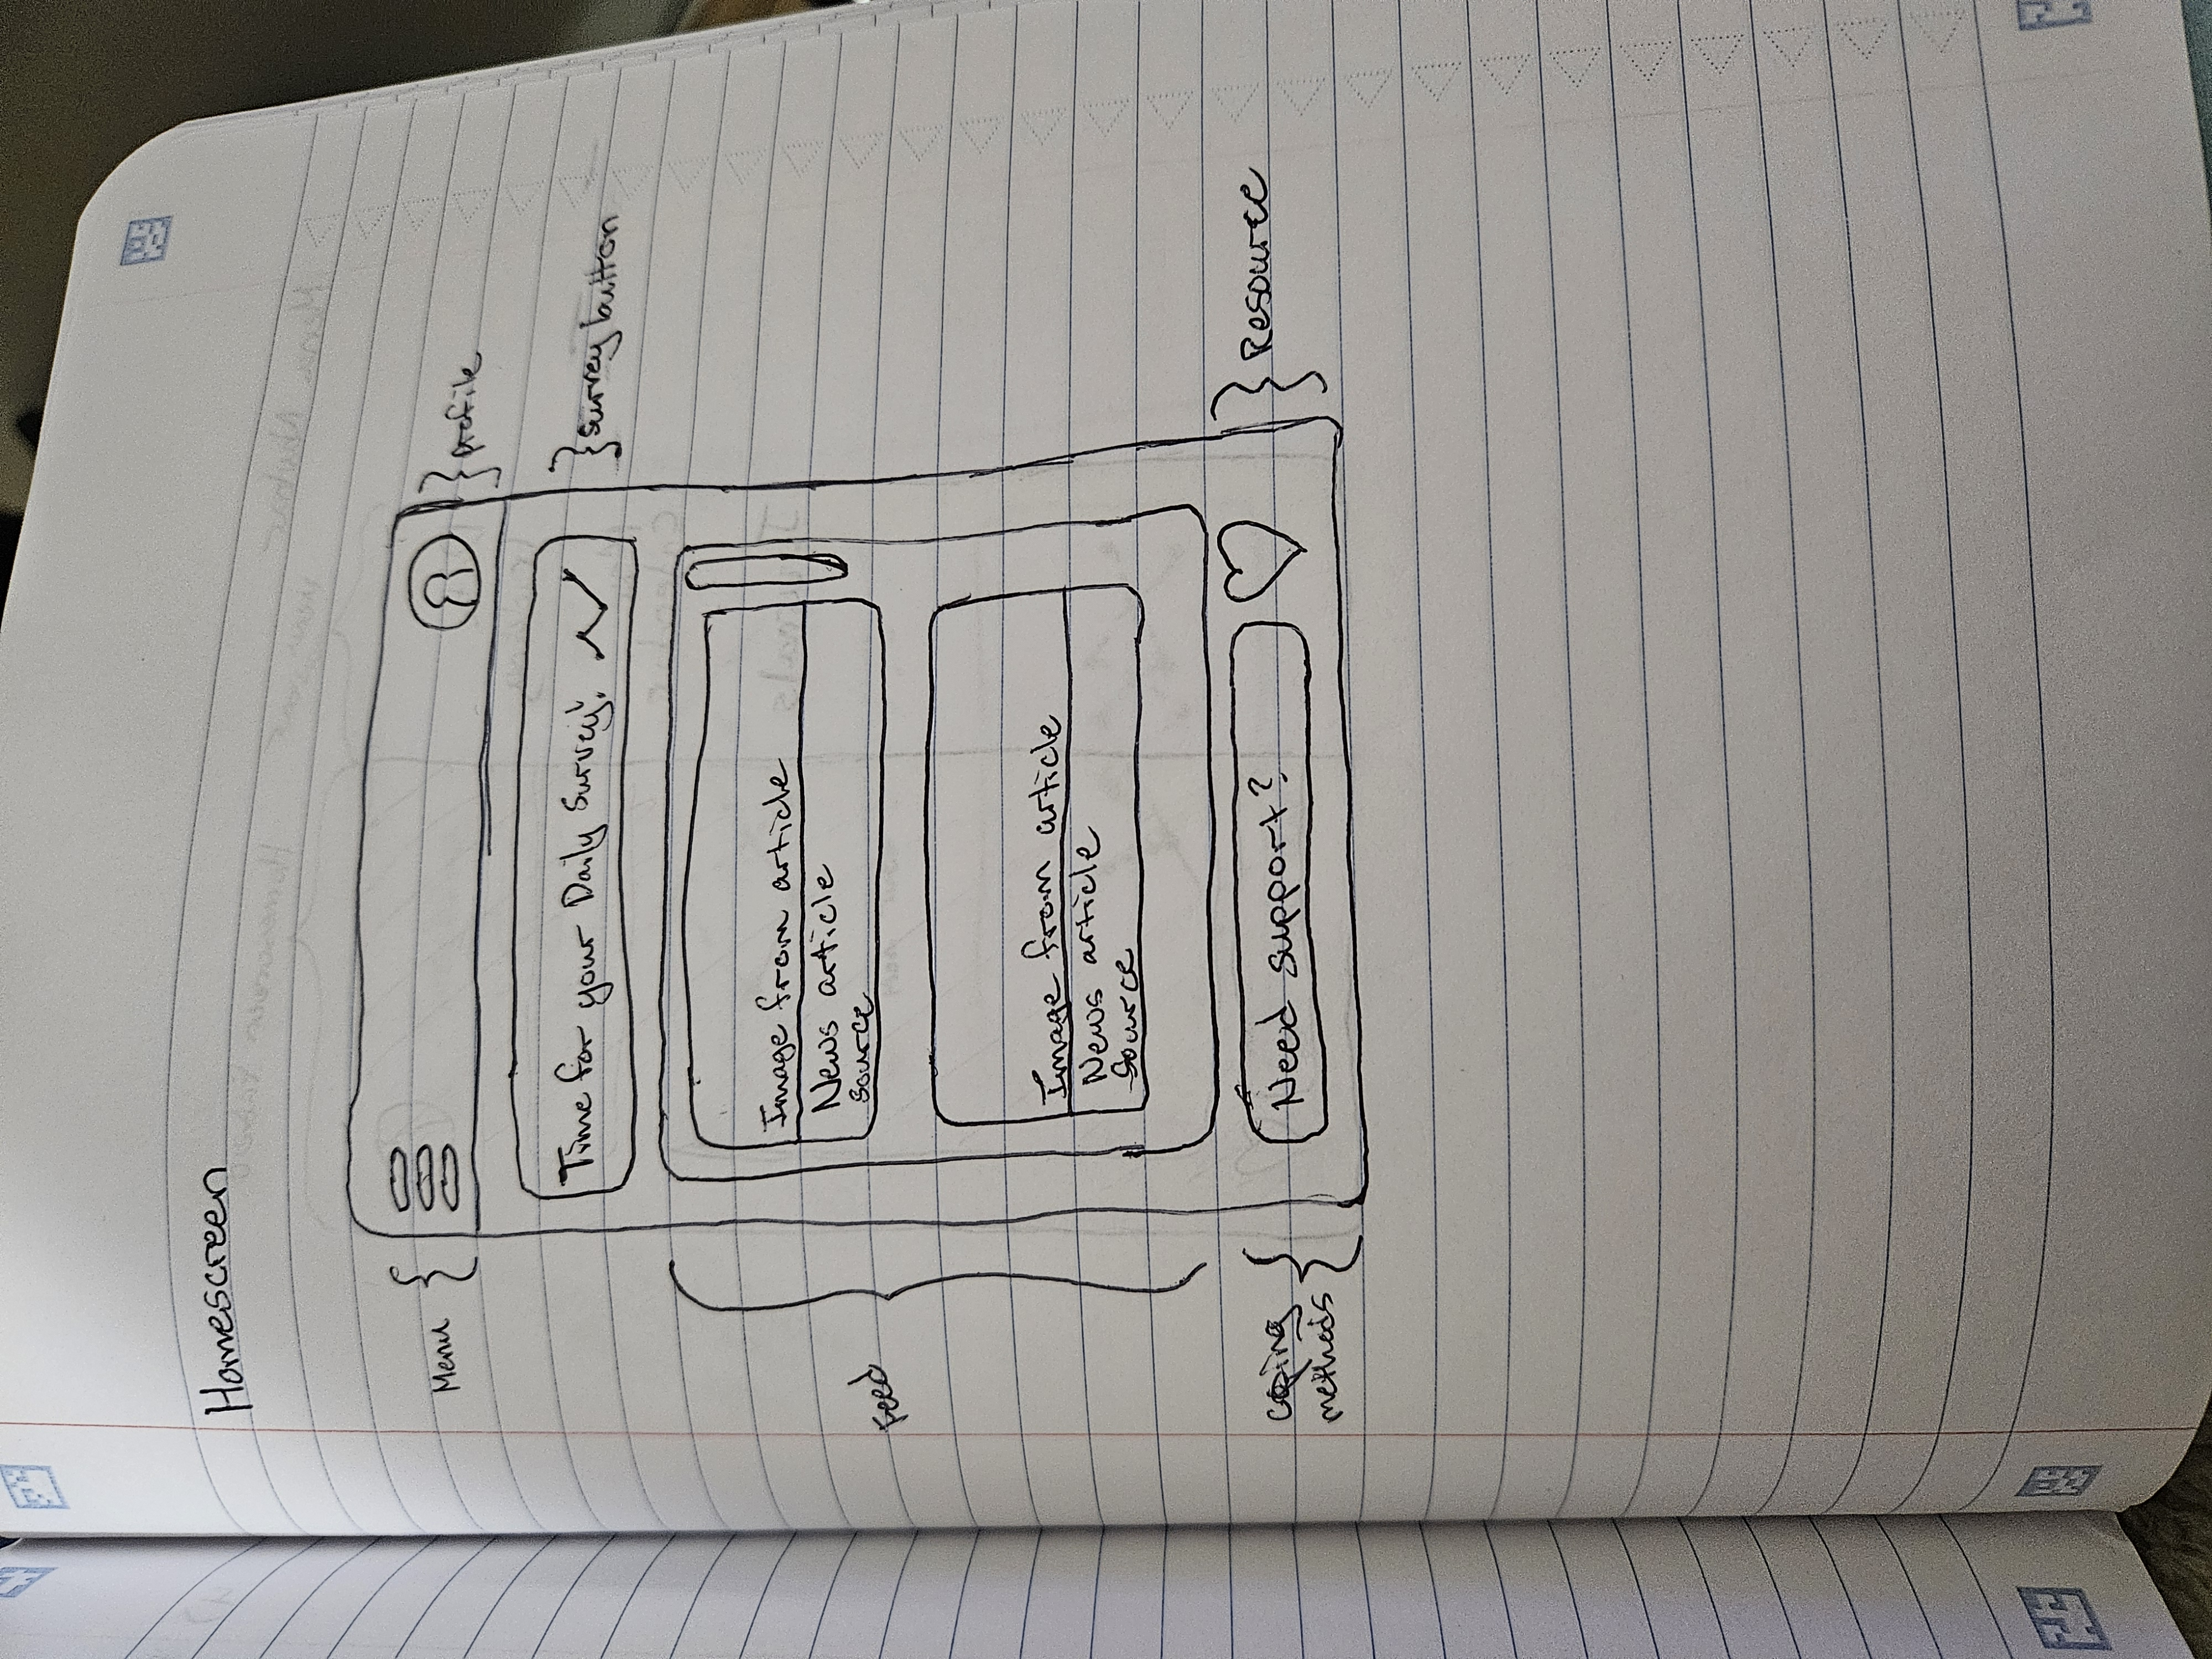
\includegraphics[scale=0.1, angle=270]{images/Homescreen.jpg}

See image for layout of homescreen. User can click the following items and achieve the following results:

Left menu button: Opens side navbar on left side of screen. This menu will include a list of further clickable links (further described in the menu section)

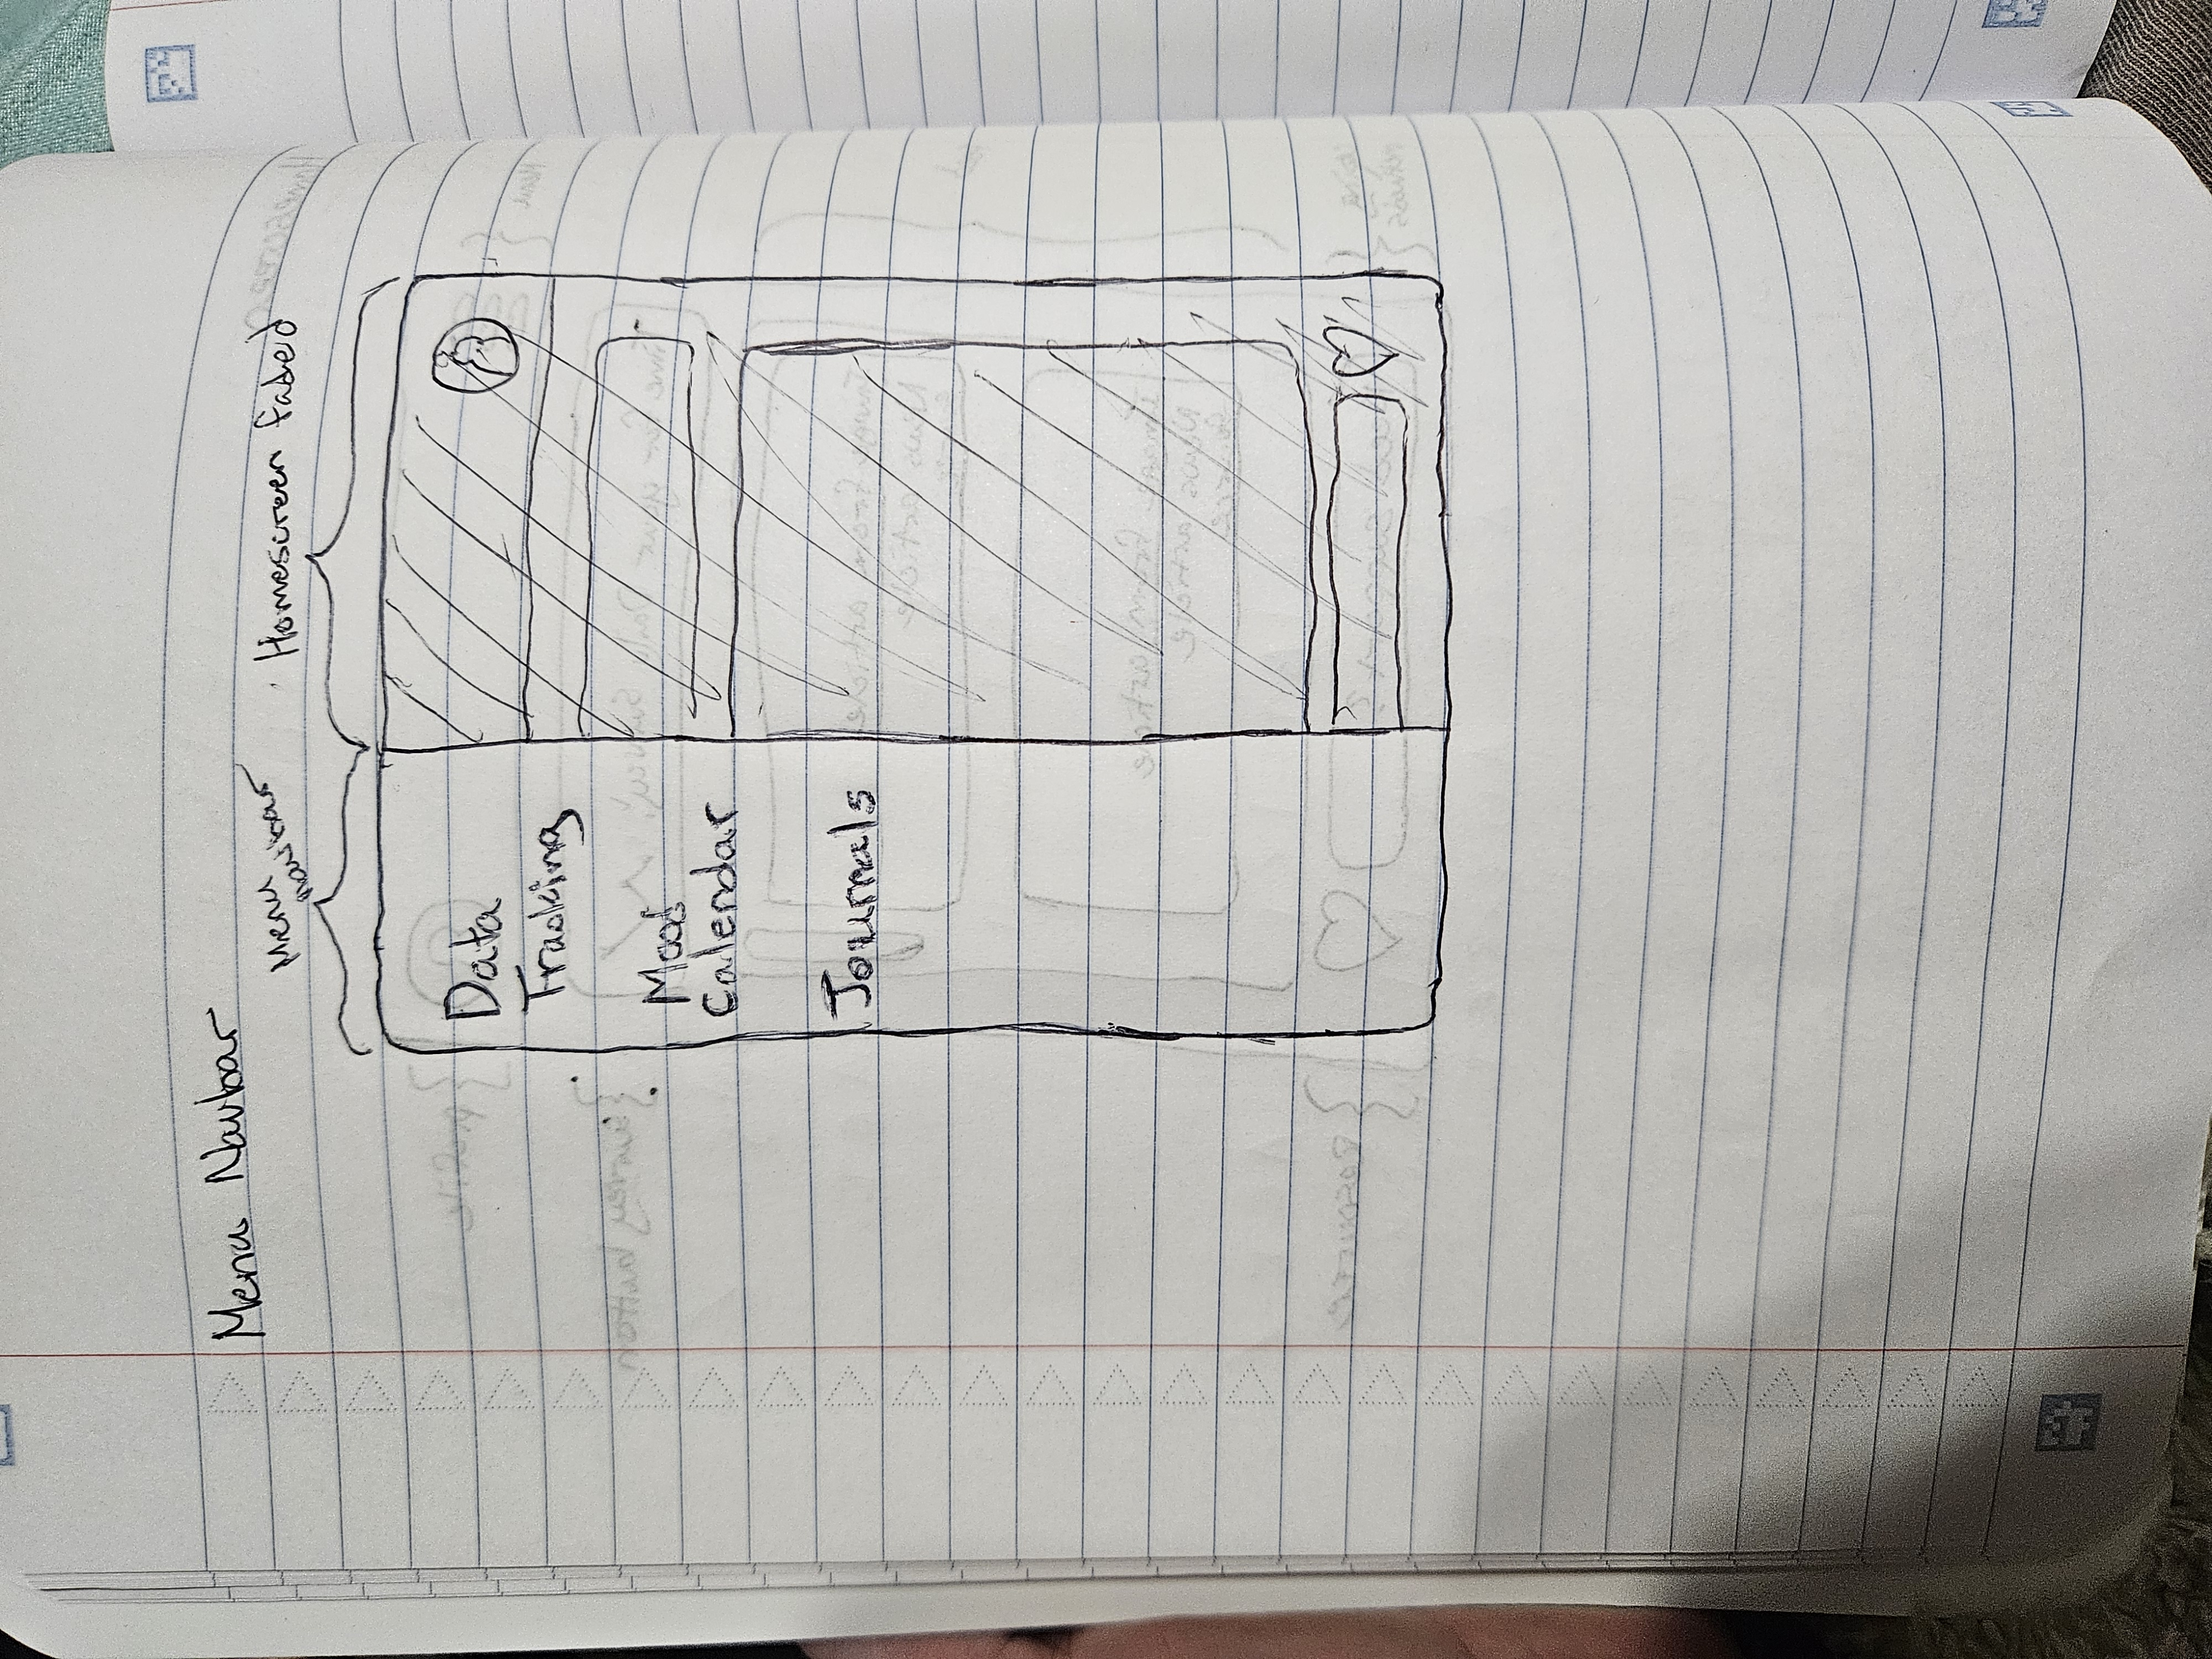
\includegraphics[scale=0.1, angle=270]{images/Menu_navbar.jpg}

Right profile button: Opens a navbar on the right, containing the user’s profile information. It will include their profile picture (clickable to allow them to change it), as well as a logout link

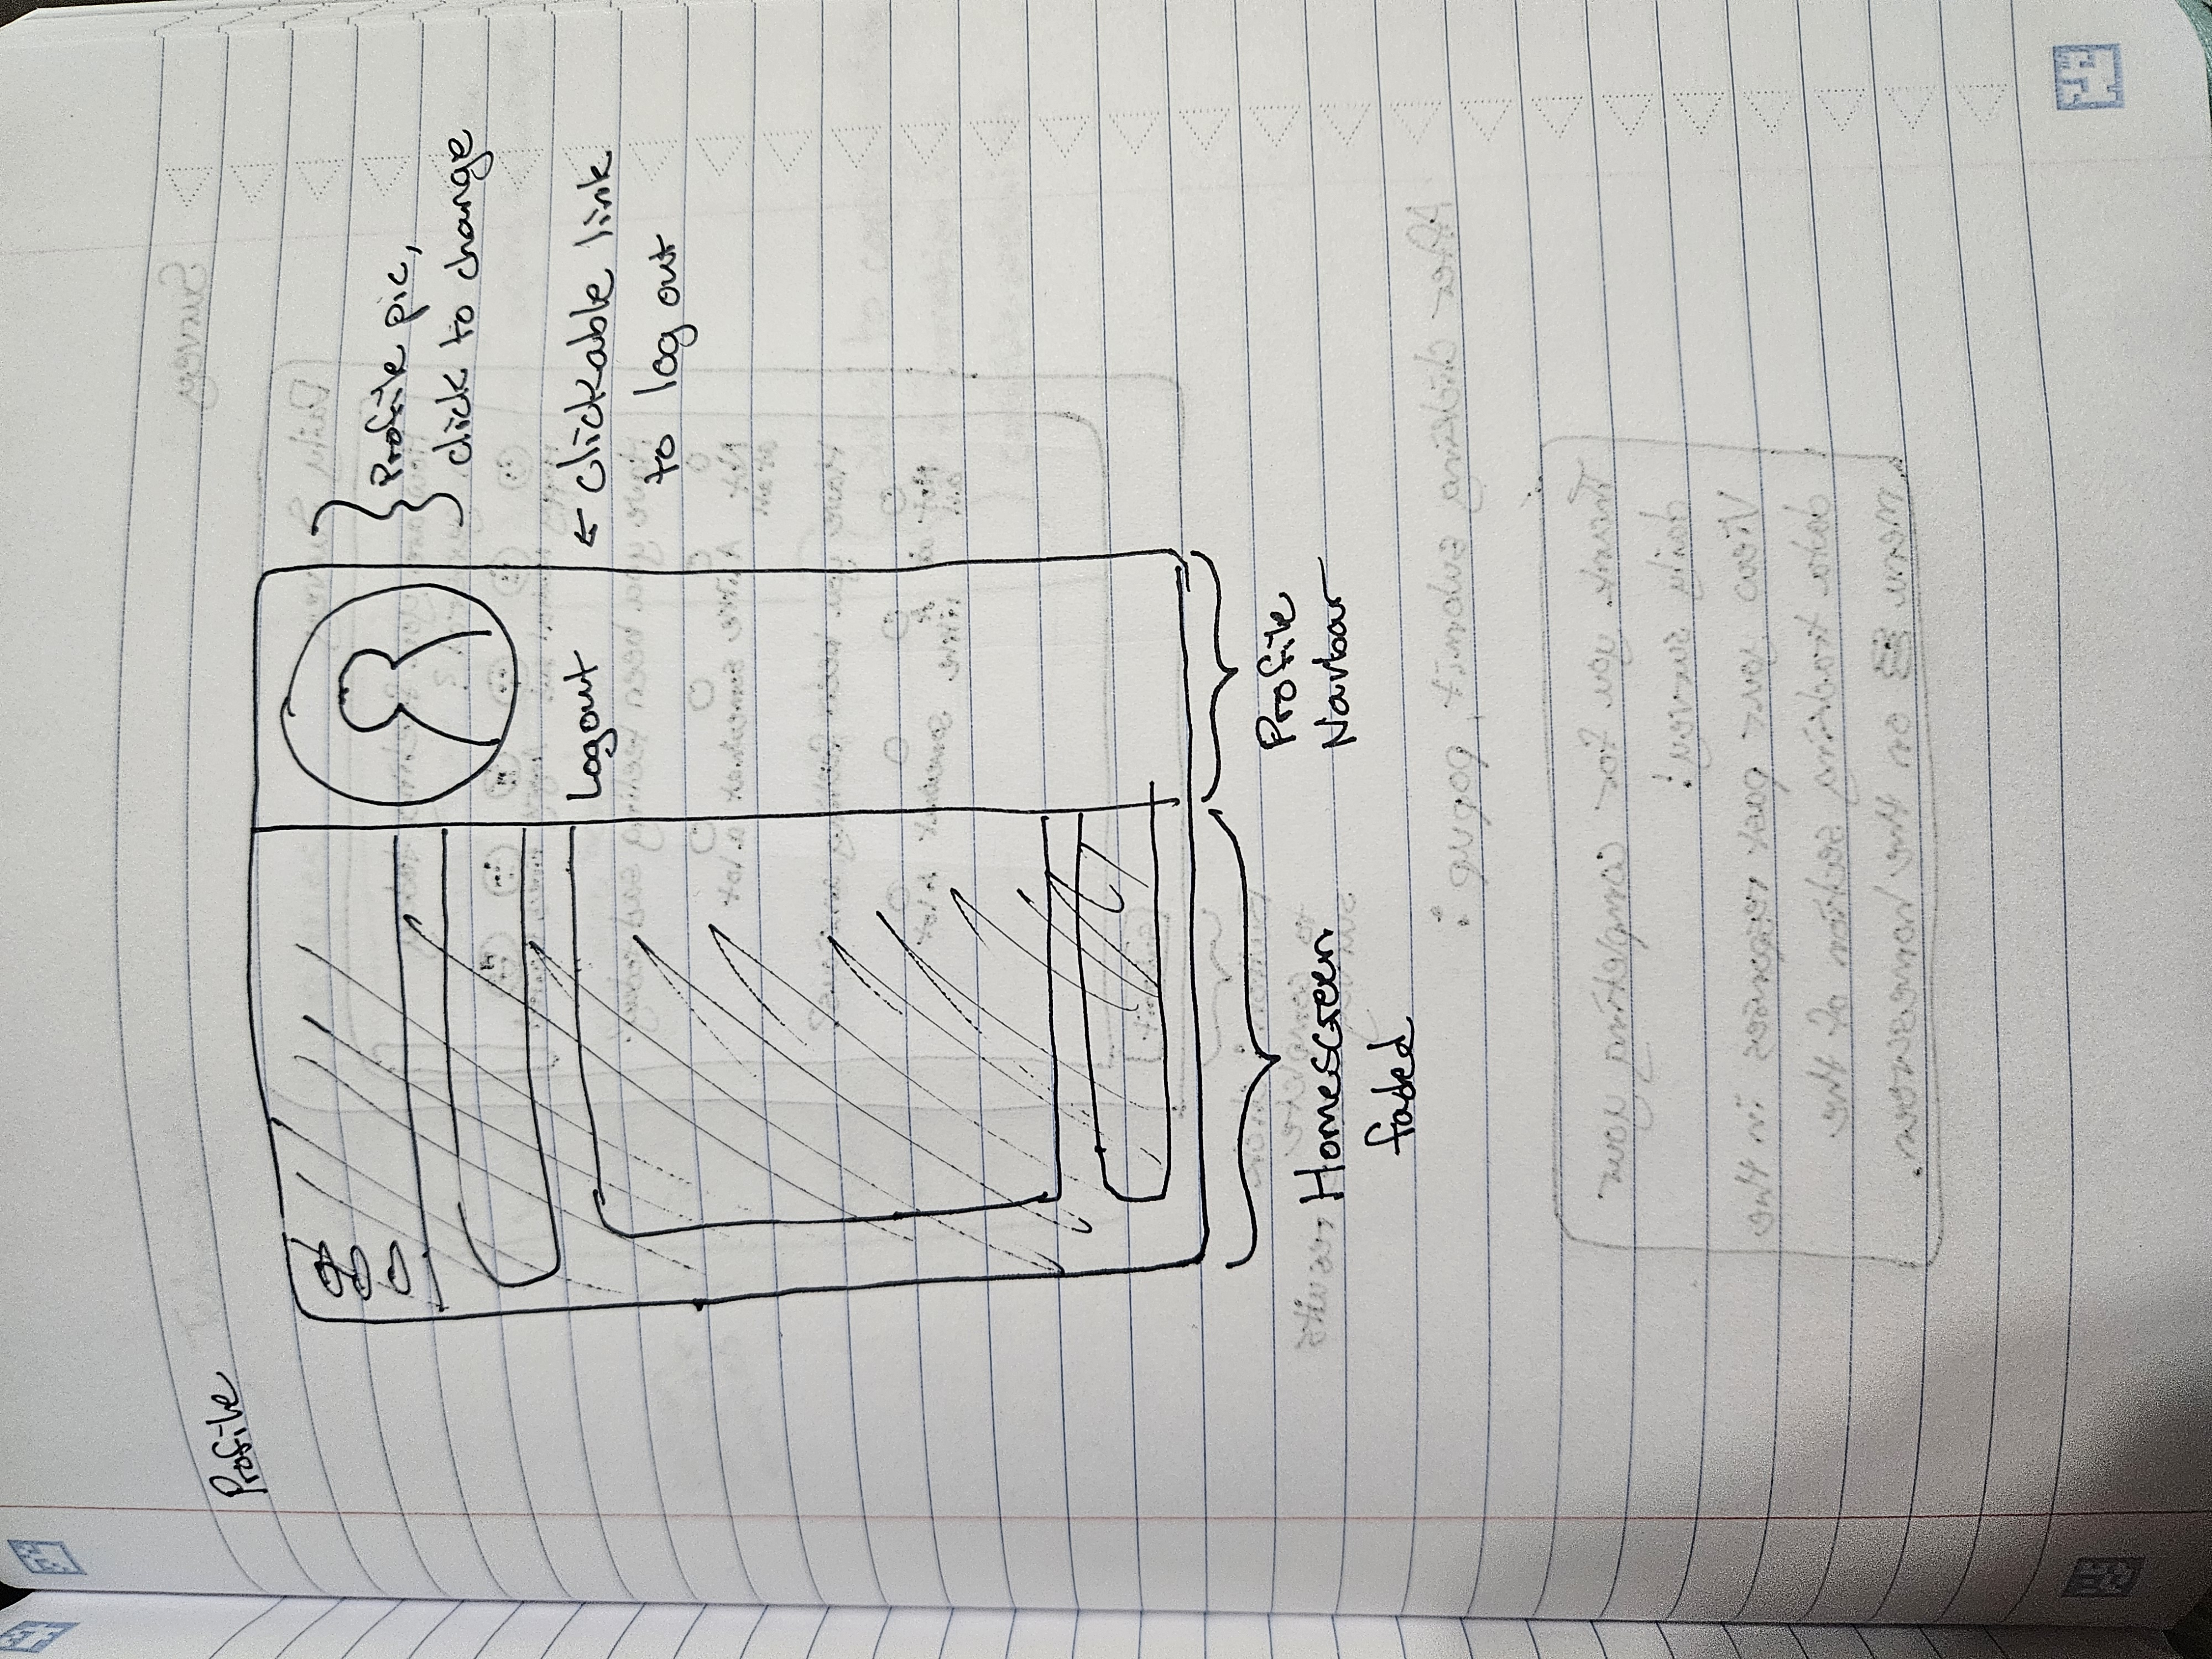
\includegraphics[scale=0.1, angle=270]{images/Profile.jpg}

Daily survey button: Clicking this button takes the user to the survey screen. The button will only appear on the homescreen if the user has not yet taken their survey for the day, and then it will disappear after the survey is completed.

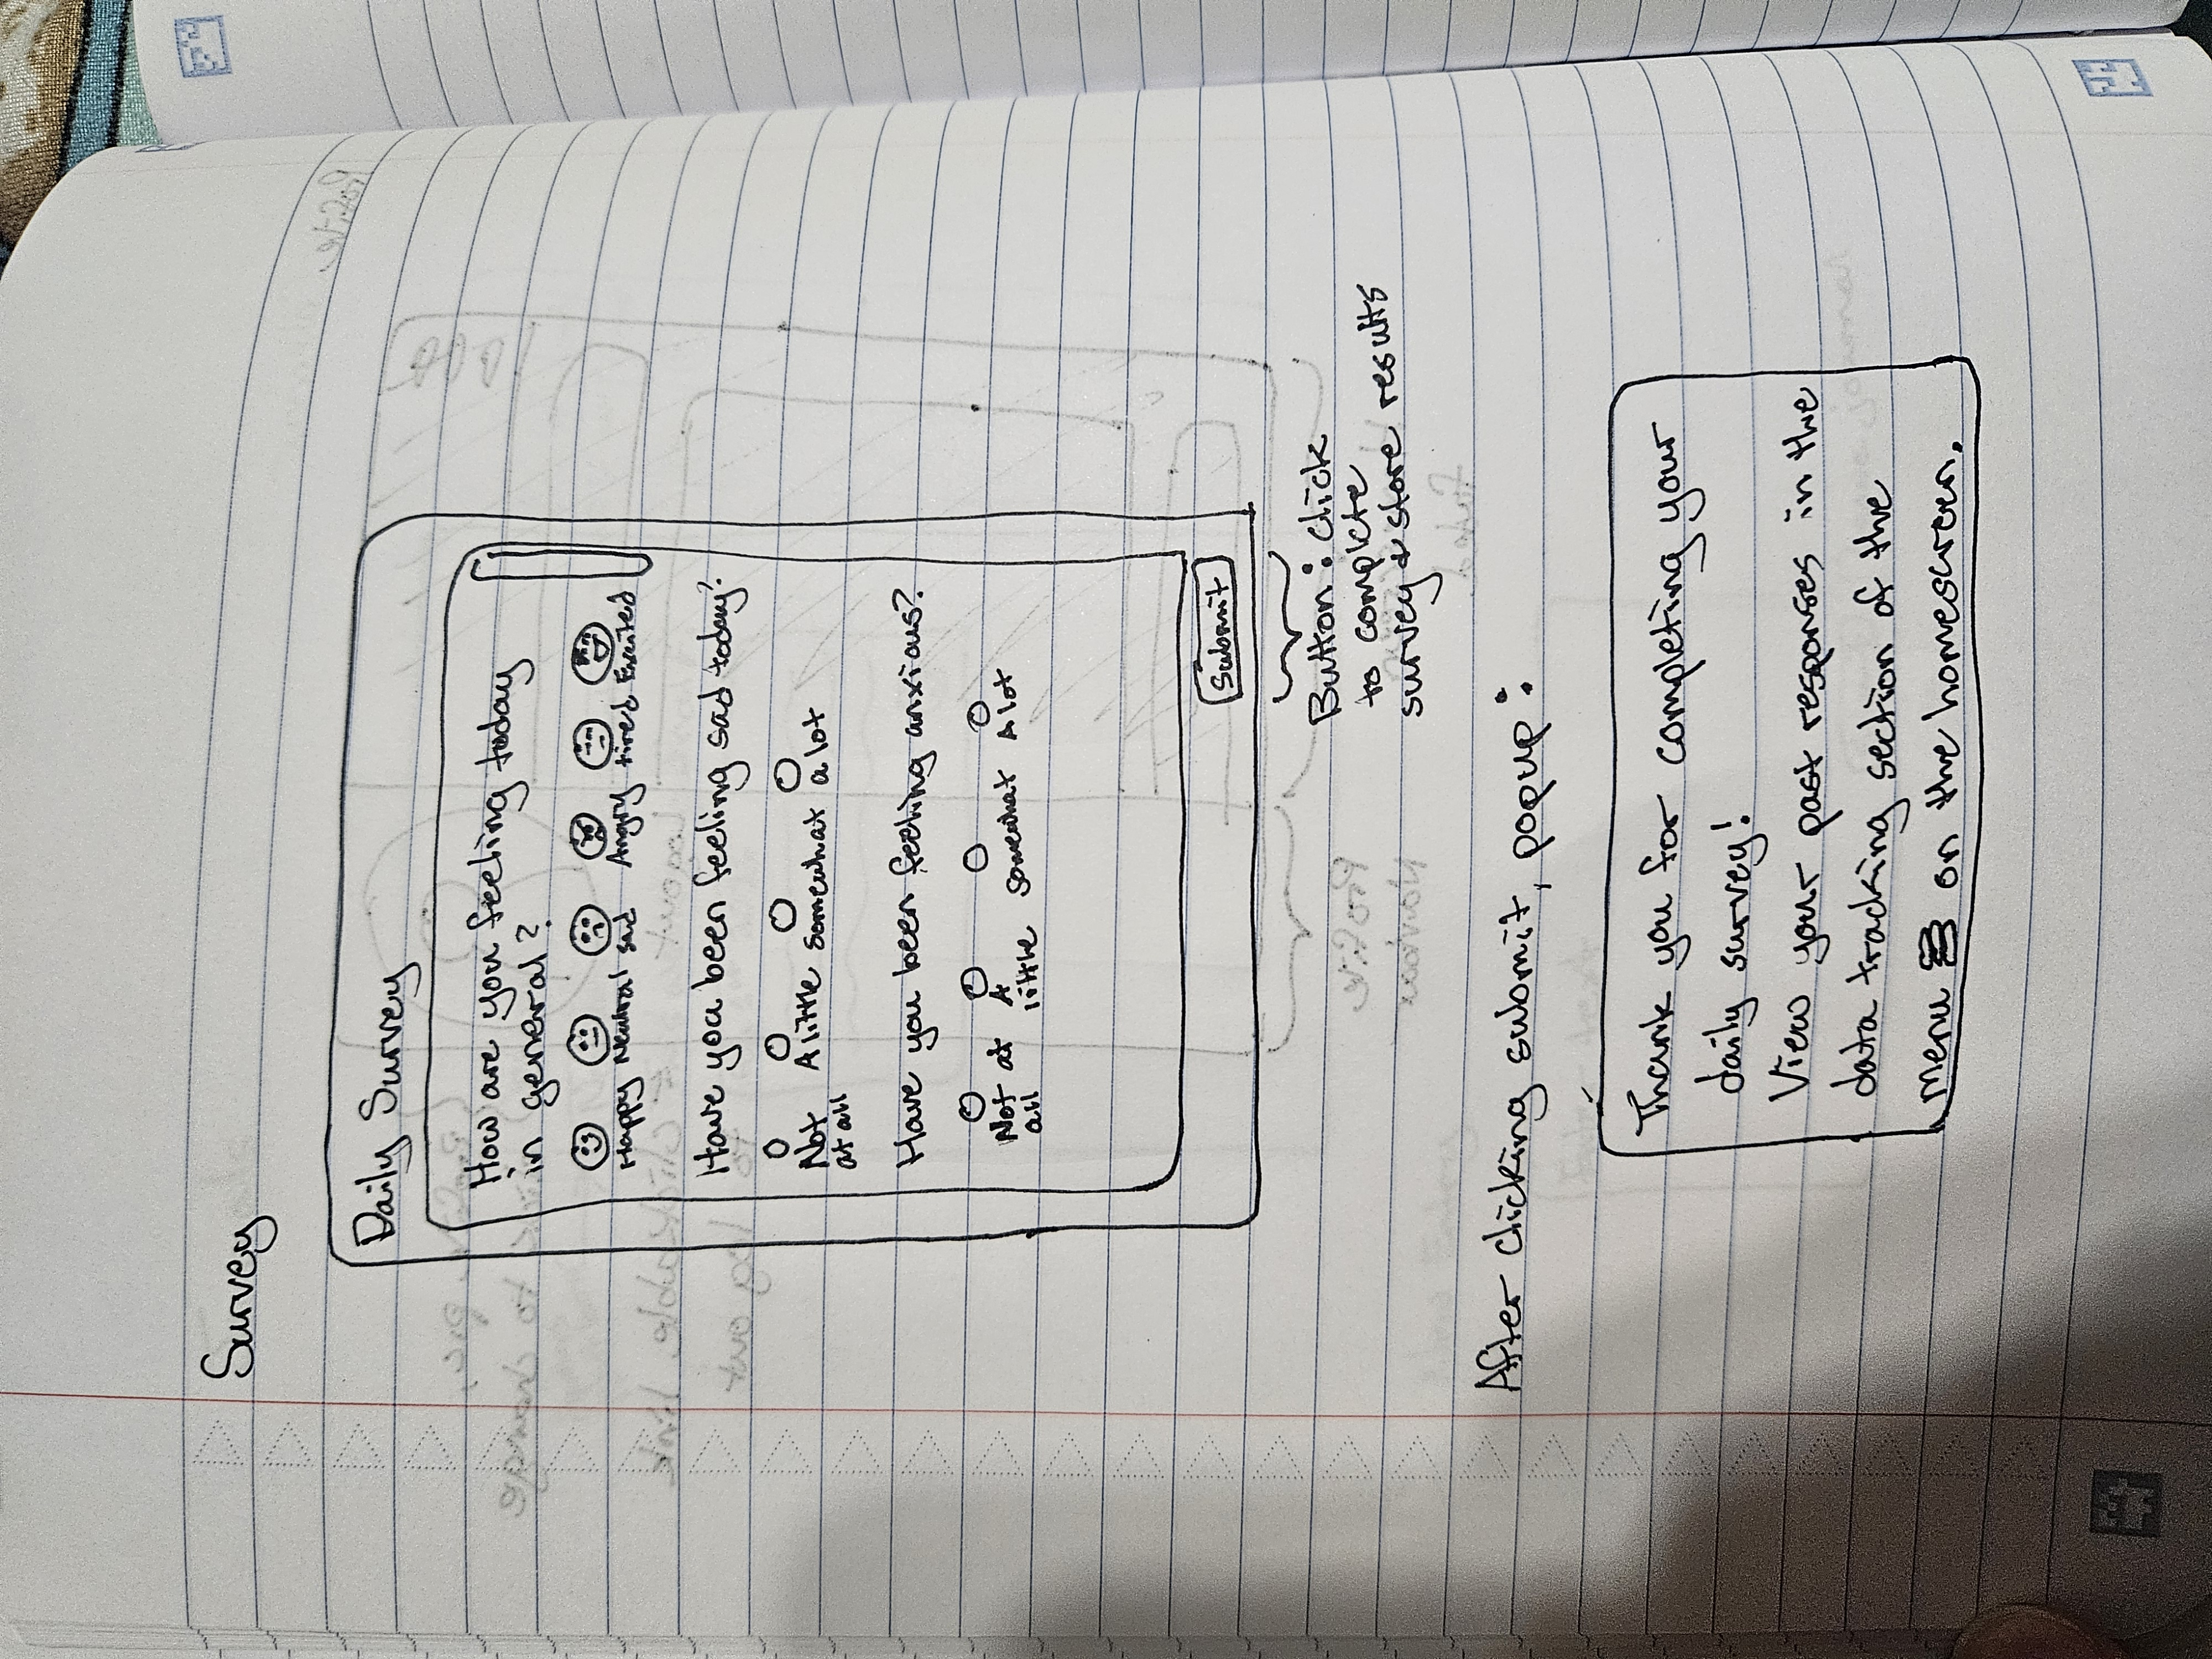
\includegraphics[scale=0.1, angle=270]{images/Survey.jpg}

Feed: Scrollable window with recommended research and news articles focused on the user’s areas of interest (they can select these from a list of choices when setting up their profile). The articles will each be in a block that will include a headline, a picture from the article (if available) and the source of the article. Clicking on an article will direct them to the article at its source online.

Coping techniques: clicking on this button will take the user to another screen within the app that will display articles about coping strategies for the symptoms the user has been experiencing or rating highly in the daily surveys. There will also be a section on this screen where the user can write down some of their own coping strategies and affirmations that will then be displayed as reminders.

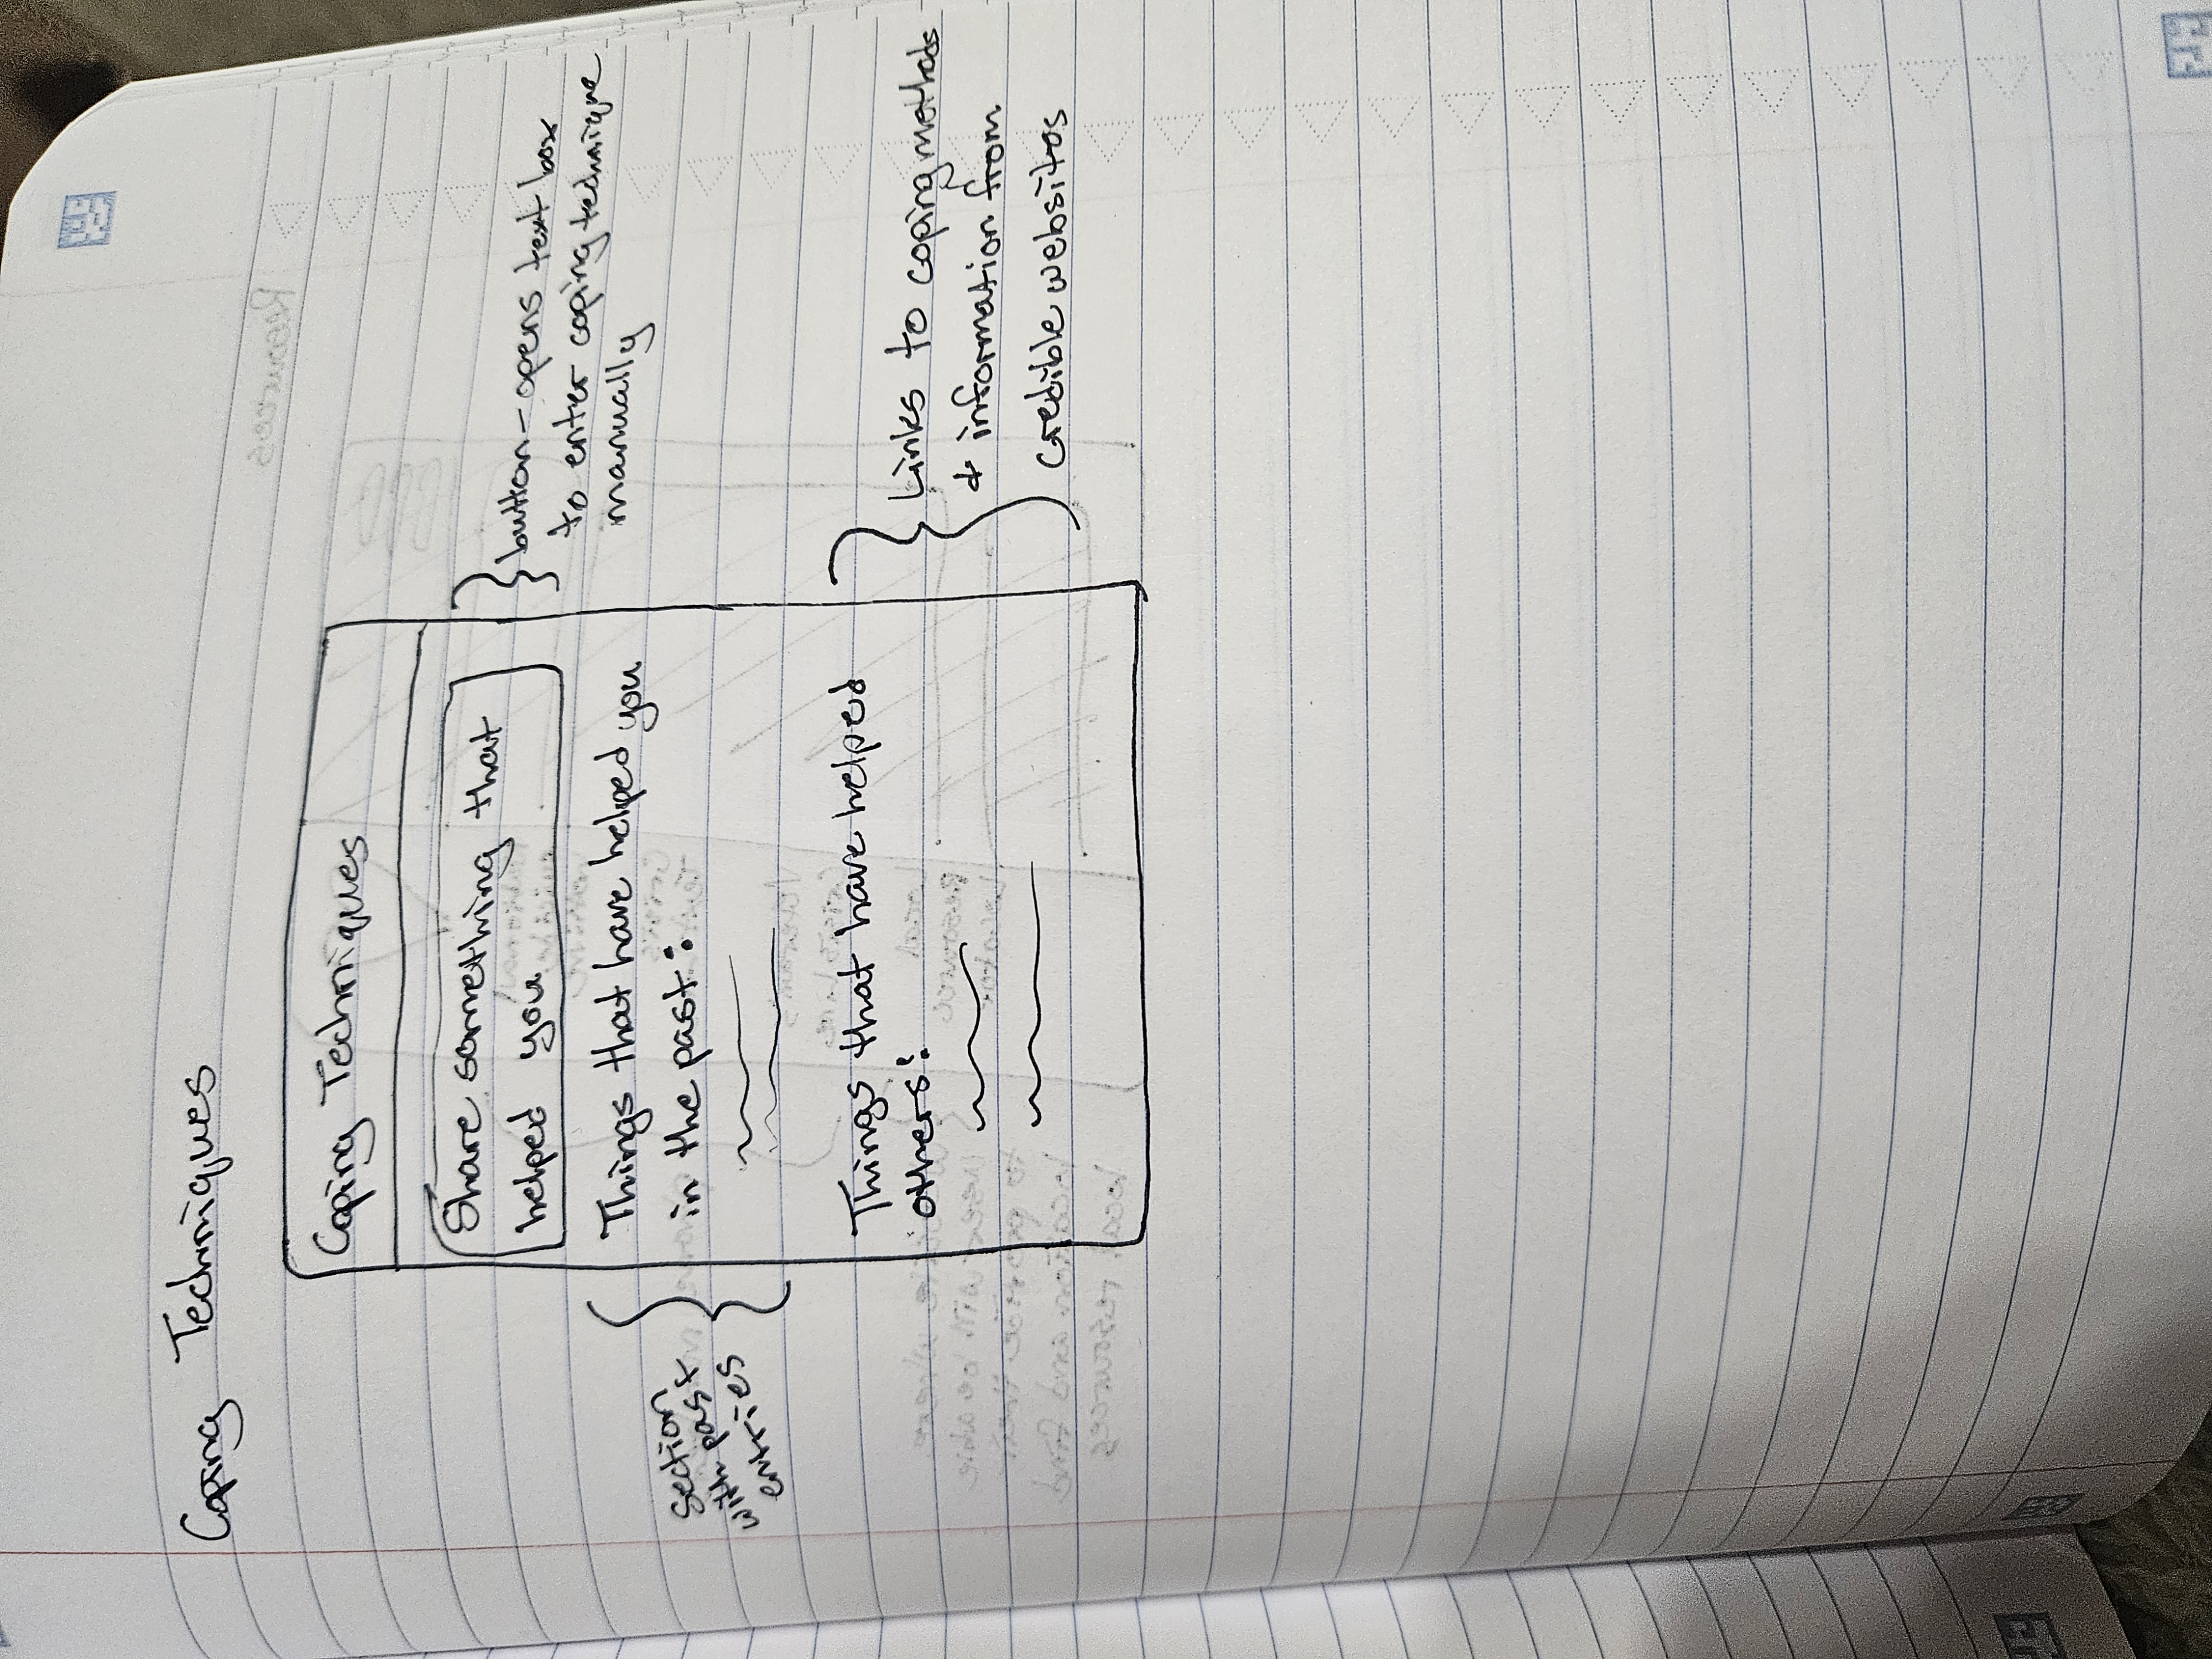
\includegraphics[scale=0.1, angle=270]{images/Coping_techniques.jpg}

Resources: Clicking the resources button will open a different right-side navbar that will include a list of resources for the user, such as hotlines for emergency support, crisis text line, warm lines for less urgent support, and national resources specific to the user’s symptoms 

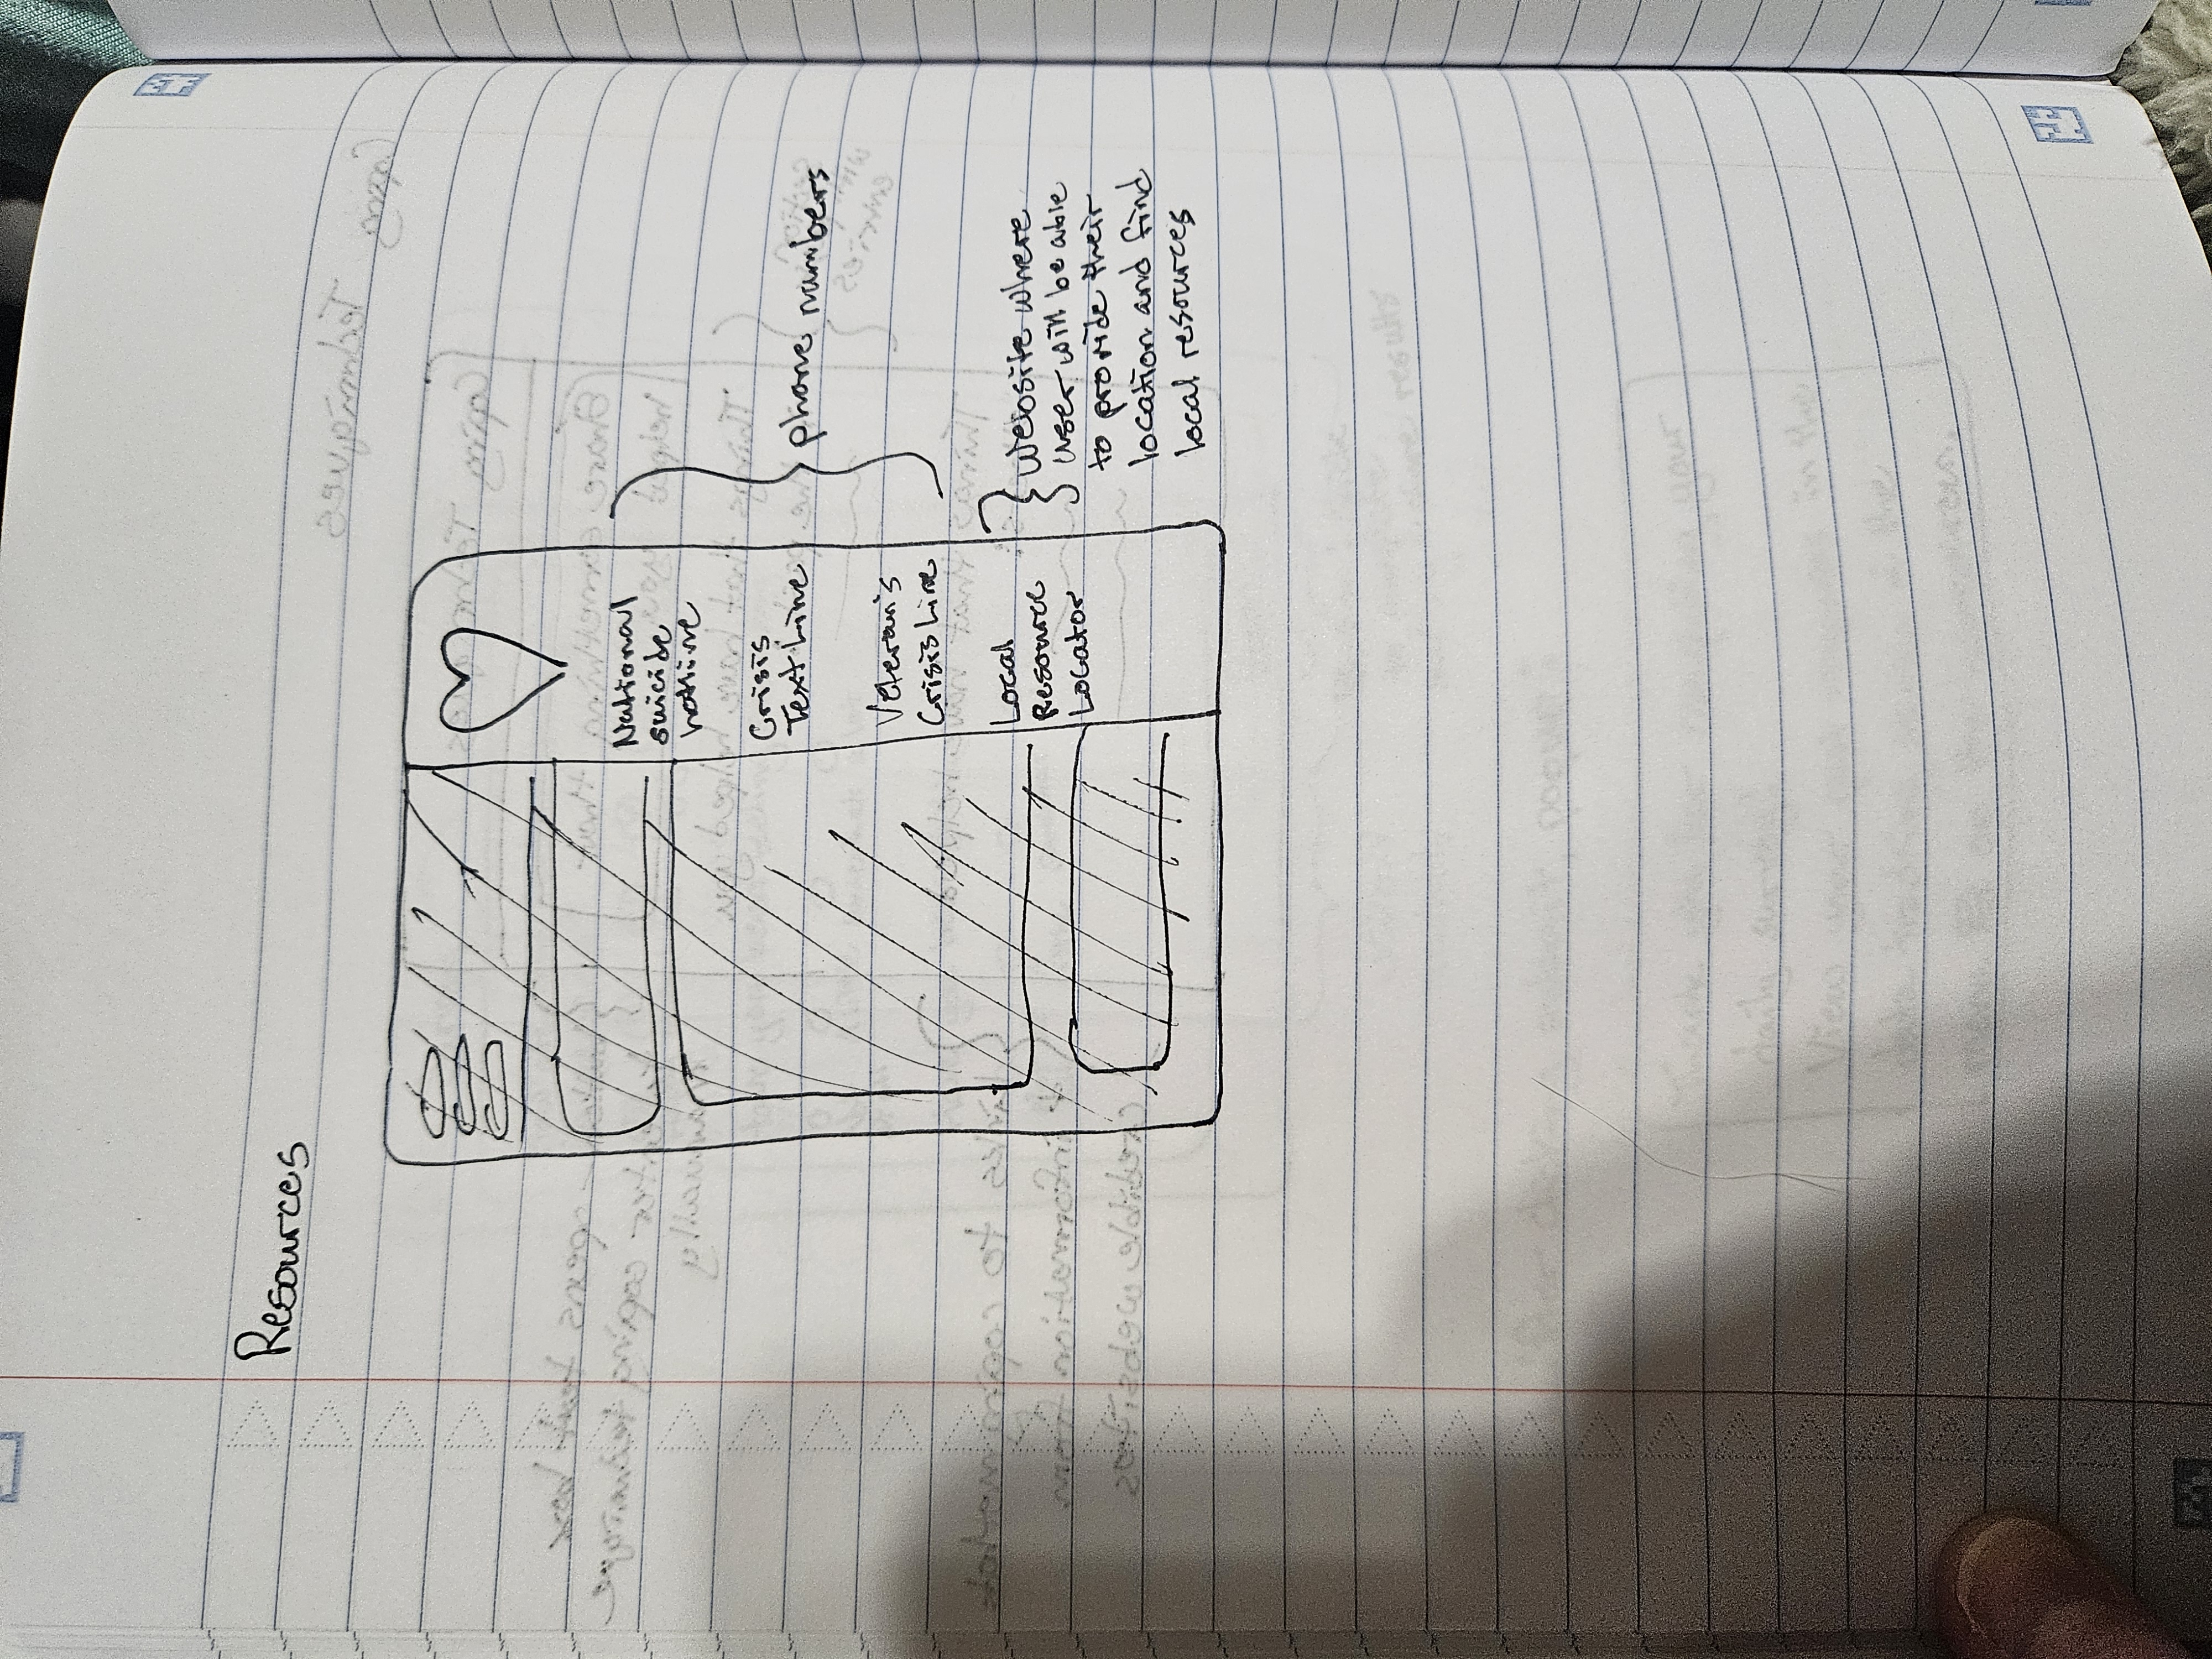
\includegraphics[scale=0.1, angle=270]{images/Resources.jpg}

Left Menu: Clicking on the three horizontal lines in the top left will open a menu navbar on the left side of the screen. The homescreen will still be visible in the background but will be faded. The menu navbar will include three clickable links: Data Tracking, Mood Calendar, and Journals. Clicking any of these links will take the user to the respective screen described below.

Data Tracking: This screen allows the user to view their past survey response data aggregated into line graphs. There are buttons at the top to change the view to weekly and monthly respectively. The top graph represents a weekly view, where each data point represents the score submitted that day over the past week. The second graph represents a monthly view, where each data point represents an average score throughout the whole month.

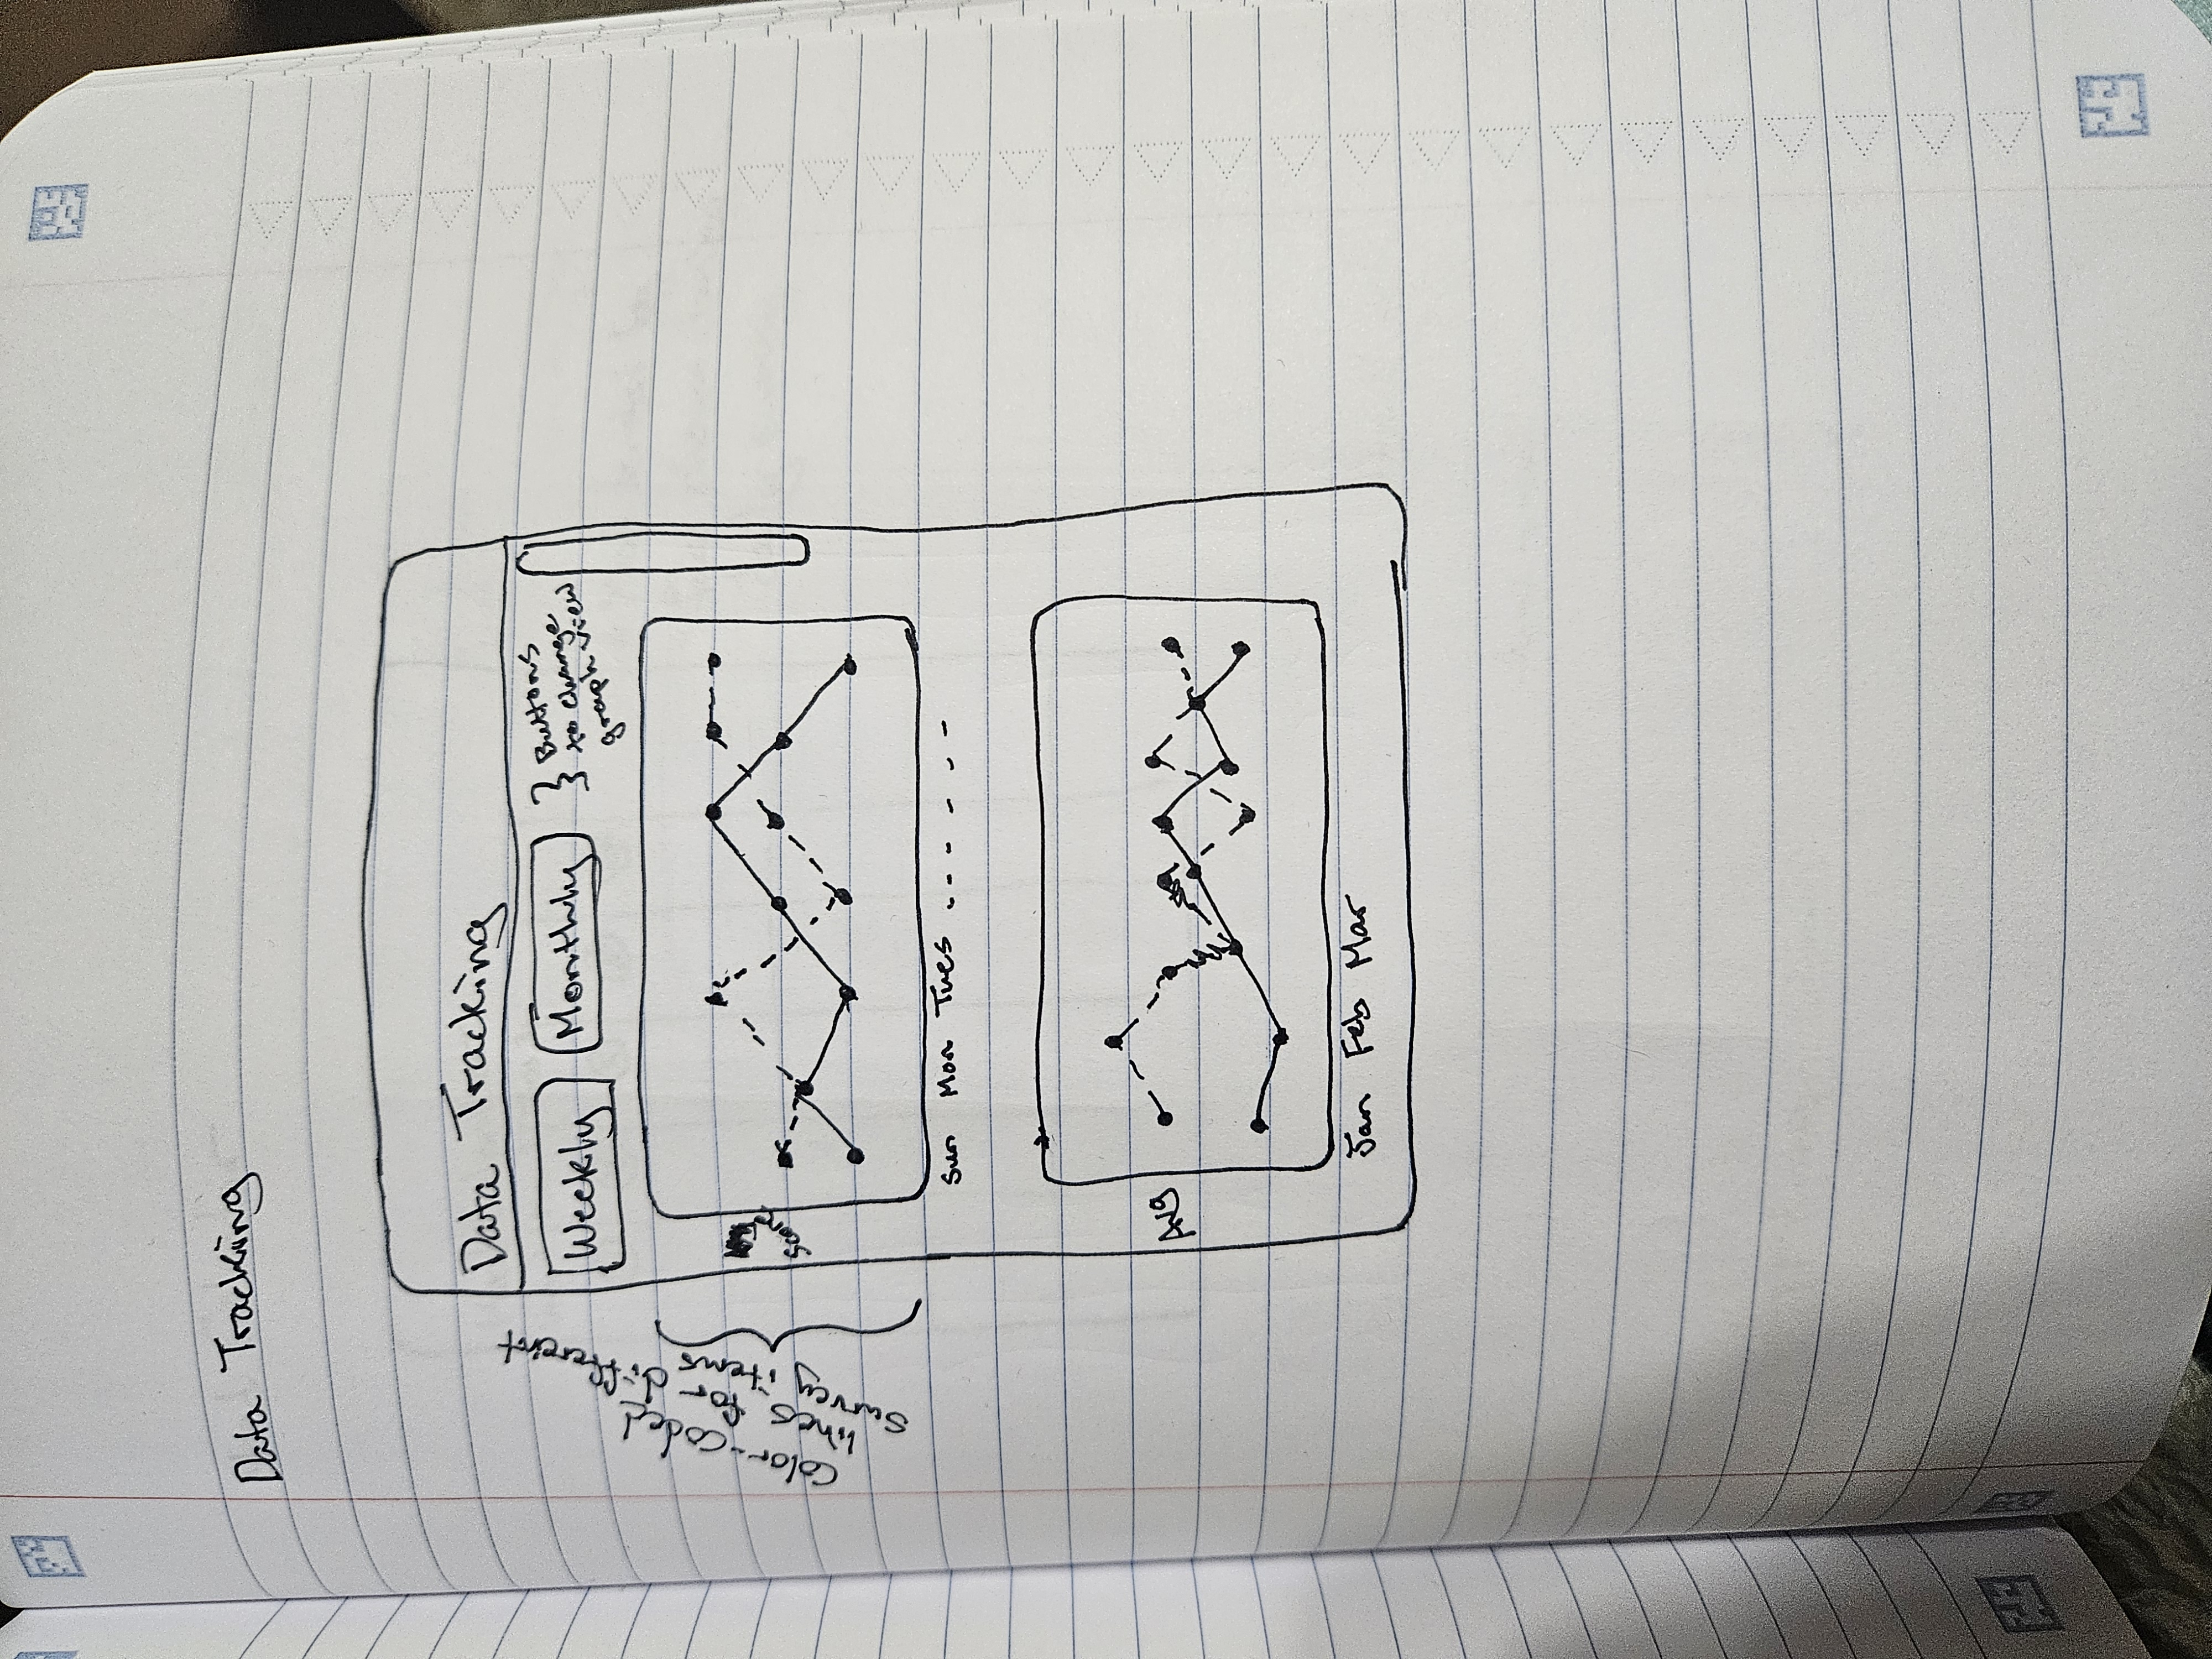
\includegraphics[scale=0.1, angle=270]{images/Data_tracking.jpg}

Mood Calendar: Clicking on the mood calendar link in the menu brings the user to this screen. They will be shown a calendar for the current month, where each day will display a symbol representing the general mood they chose for that day in their daily survey.

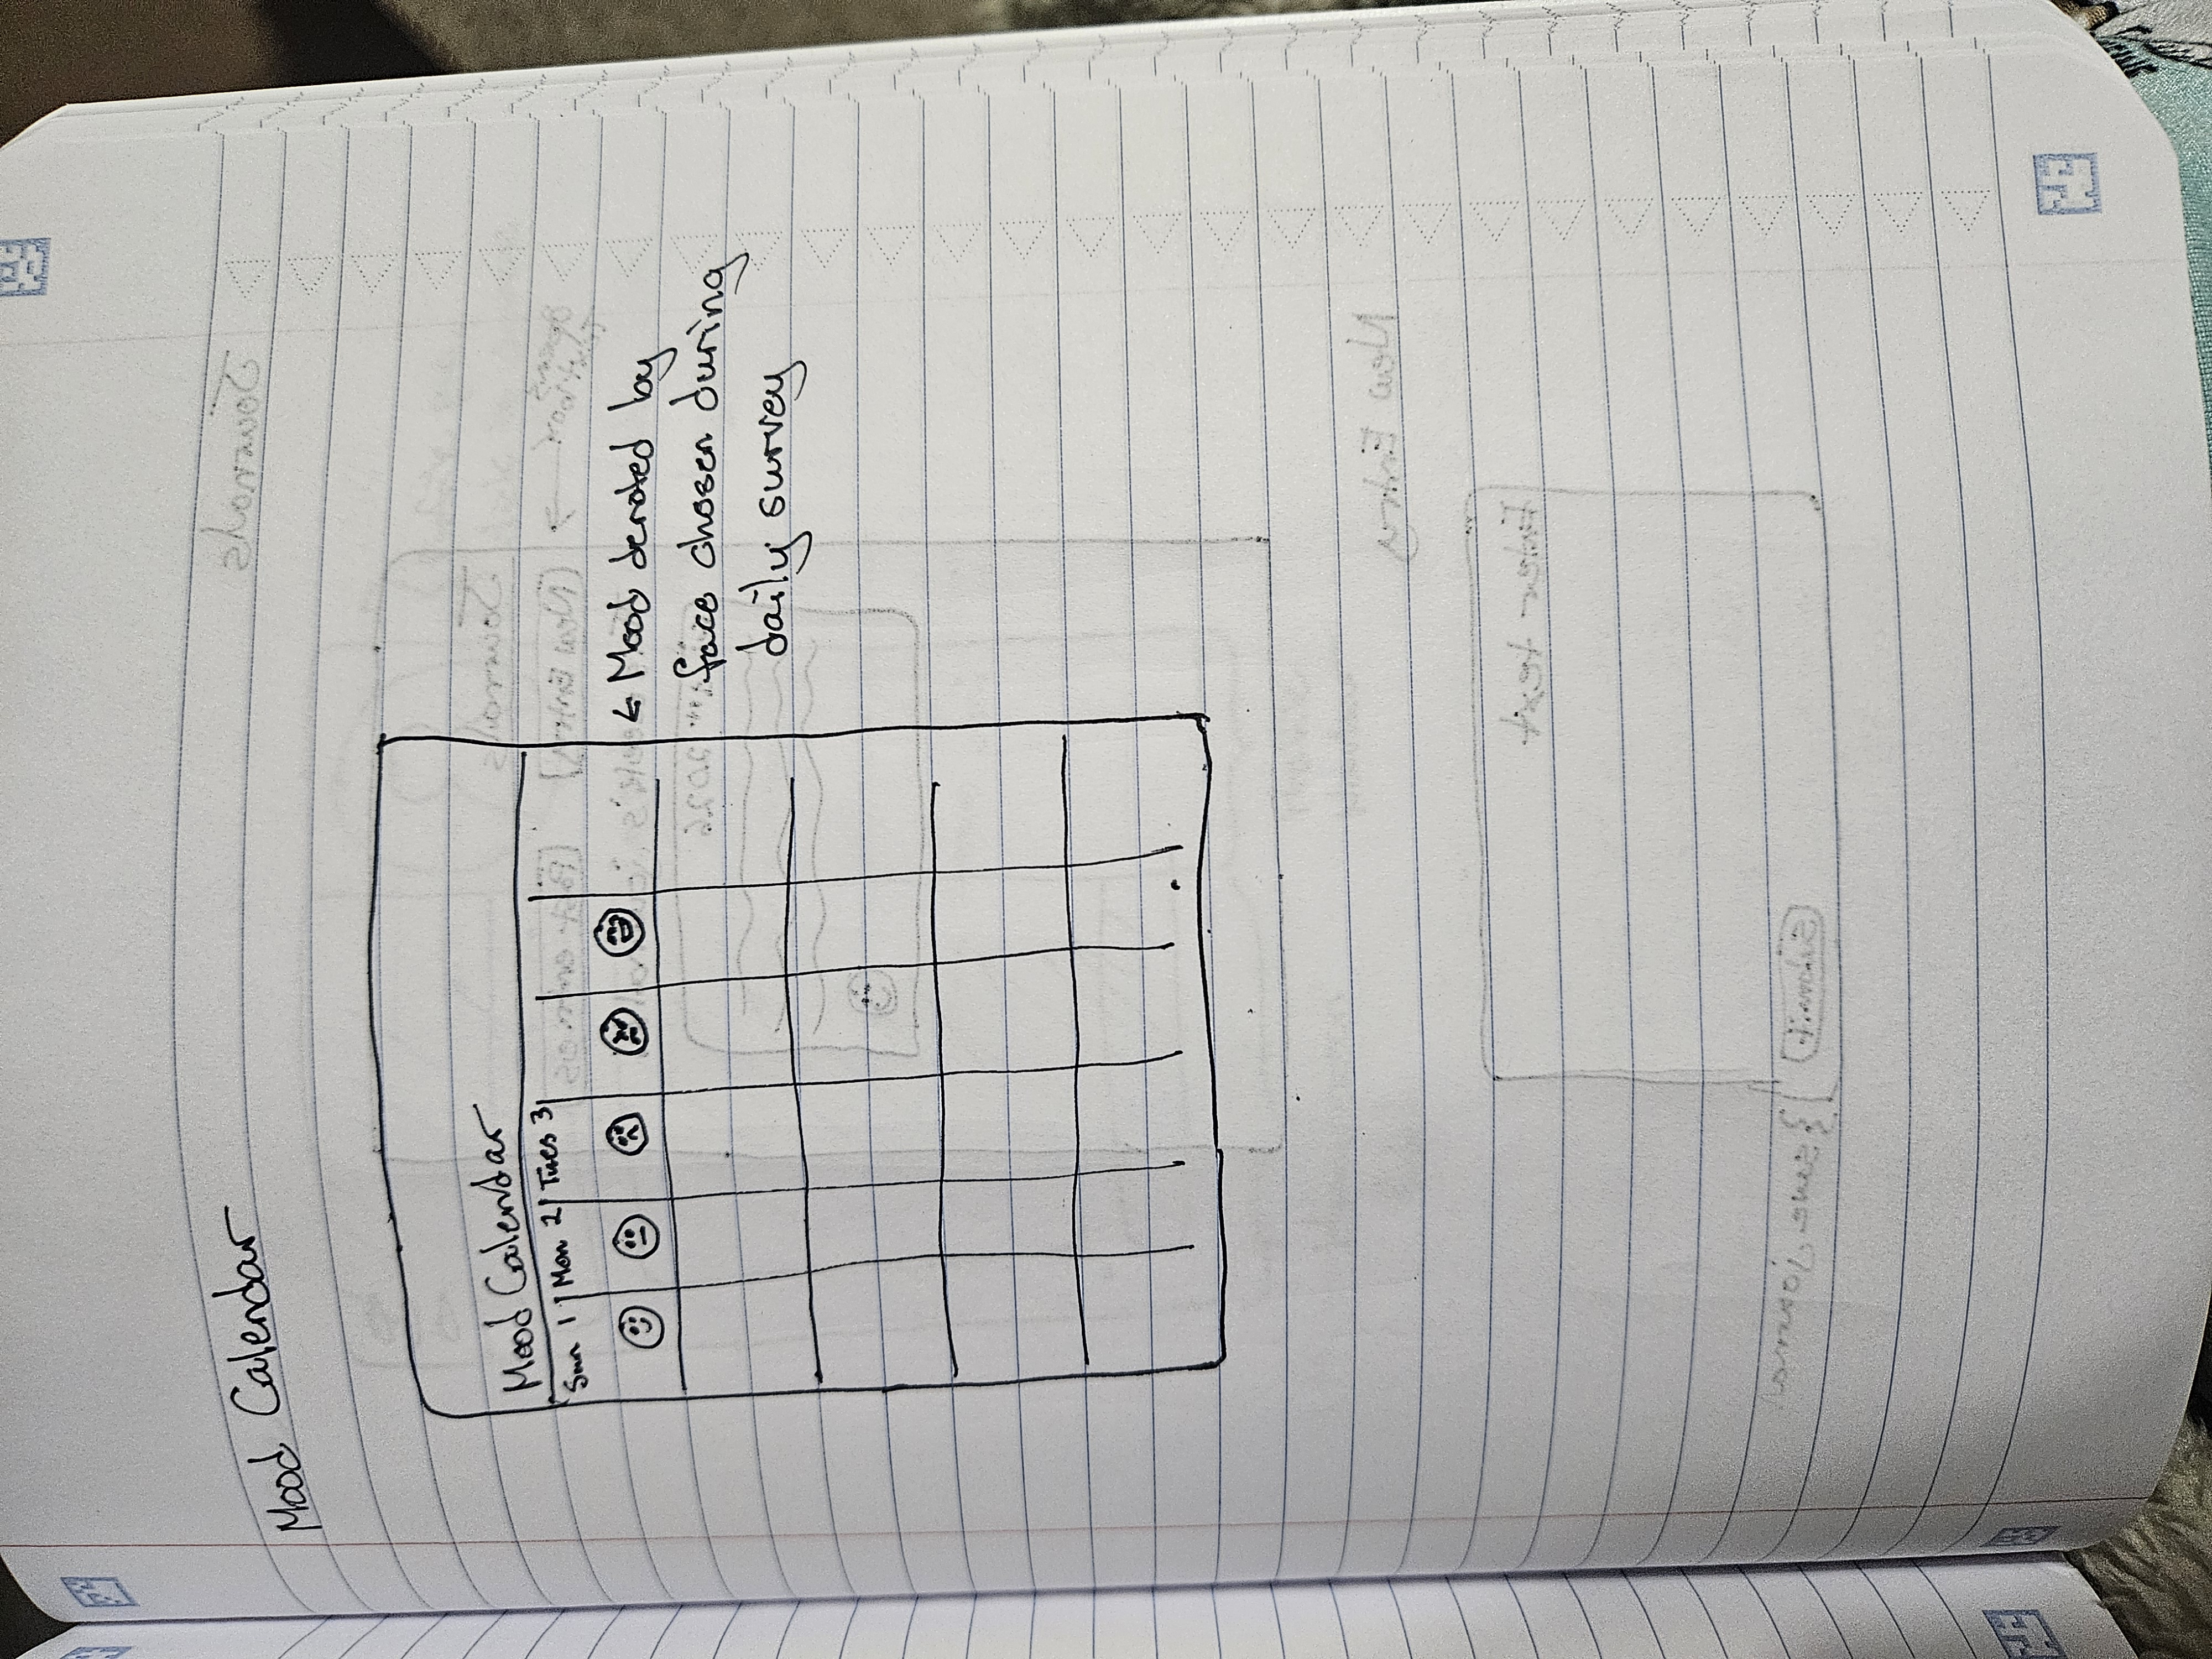
\includegraphics[scale=0.1, angle=270]{images/Mood_calendar.jpg}

Journals: Clicking on the Journals link in the menu brings the user to this screen. There are buttons to both create new journal entries and view past entries. Clicking on the new entry button will open a text box for the user to type in. The remainder of this screen is dedicated to past responses, which will also include the date the response was submitted. Clicking the past entries button will open a scrollable list of timeframes the user can choose from, including the past week and a specific month and year. Their selection will dictate which entries are displayed in the bottom half of the screen.

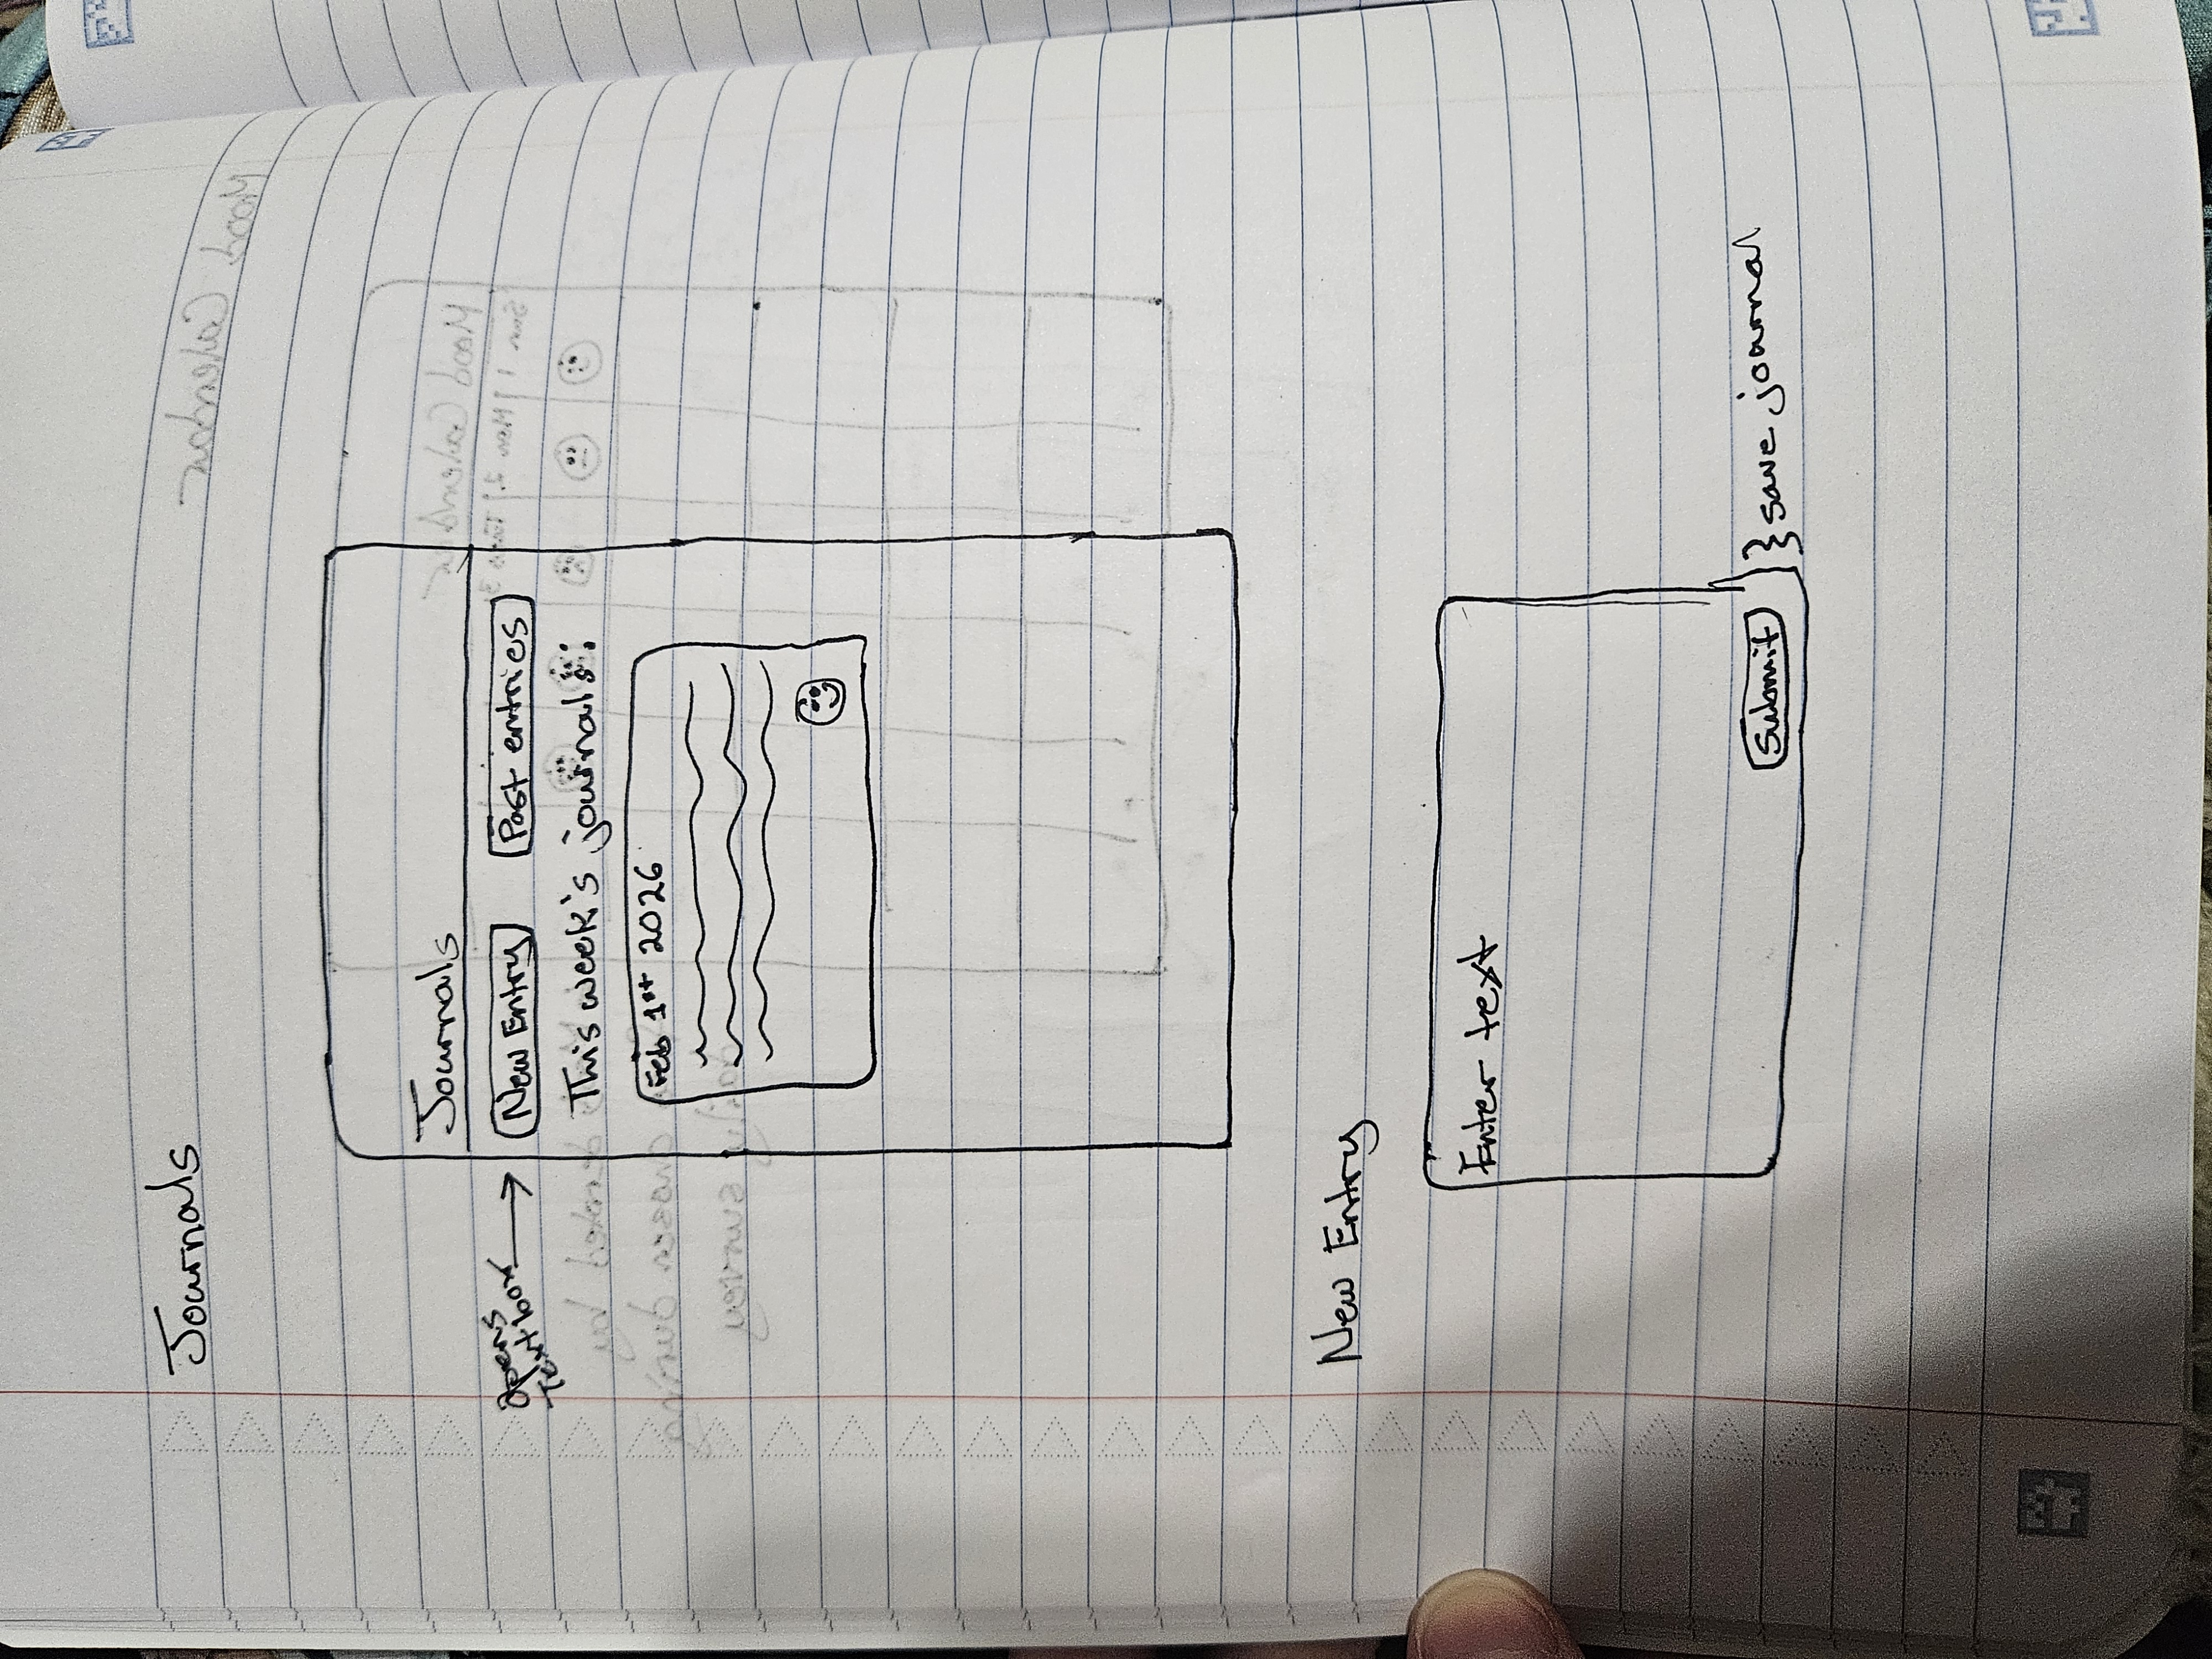
\includegraphics[scale=0.1, angle=270]{images/Journals.jpg}

Right Profile: Clicking the circle in the top right of the homescreen will open a navbar on the right. As with the menu, opening this navbar will fade the rest of the homescreen. On this navbar the user will see a larger version of the image they clicked on to get here: their profile picture. Clicking on this larger profile picture will give them the option to change it. There is also a logout link beneath the profile picture, which the user can click on to sign out of their account.

Survey: The survey button can be found on the homescreen just below the top navbar if the user has not yet taken their daily survey. If they have already taken their survey, the button will disappear until the next day. Clicking the button brings the user to the survey screen, where they will be presented with the same survey questions as always, with a submit button in the corner that can be clicked to submit their responses and close the survey.

Coping Techniques: The coping techniques button can be found at the bottom left of the homescreen. Clicking it will bring the user to the coping techniques screen. At the top of this screen the user will see a button that opens a text box, allowing the user to submit coping techniques that have worked for them in the past in an open-ended response. These responses are then displayed in a section below the button to remind the user of things that have helped them in the past. Below this section, at the bottom of the screen, the user can find a section devoted to credible websites where they can find further suggested coping methods they can try.

Resources: Clicking on the heart button on the bottom right of the homescreen opens the resources menu, a navbar on the right side of the screen. This navbar will feature a list of phone numbers the user can call in an emergency, as well as a local resource locator, which brings the user to an outside website where they can specify their location and find local resources.



\end{document}
